%!TEX program = xelatex
% 完整编译方法 1 pdflatex -> bibtex -> pdflatex -> pdflatex
% 完整编译方法 2: xelatex -> bibtex -> xelatex -> xelatex
\documentclass[lang=cn, 11pt]{elegantpaper}

\title{第一次作业}
\author{\href{https://ddswhu.me/}{邓 东 升}}
%\institute{\href{https://elegantlatex.org/}{Elegant\LaTeX{} 项目组}}
\date{\today} 

\newtheorem{lizi}{\heiti }
\renewenvironment{proof}{\noindent{\heiti 证}\quad}{\quad \hfill$\Box$\vspace{2ex}}
\newcommand{\jieda}{\noindent{\heiti 解}\quad}

\usepackage{tikz}            %画图
\usetikzlibrary{positioning, math} 

\tikzset{
MyNodeStyle/.style  ={ every node/.style= {circle, draw,  
                                                             fill=black, 
                                                             %line width=2pt,
                                                             inner sep=0pt, 
                                                             minimum width=3pt},
                                  node distance=2cm},
MyEdgeStyle/.style  ={very thick},
LoopA/.style={to path={
                     .. controls +(60:1.5) and +(150:1.5) .. (\tikztotarget) \tikztonodes}},
LoopD/.style={to path={
                     .. controls +(220:1.5) and +(310:1.5) .. (\tikztotarget) \tikztonodes}},
LoopL/.style={to path={
                     .. controls +(140:1.5) and +(220:1.5) .. (\tikztotarget) \tikztonodes}},
LoopR/.style={to path={
                     .. controls +(330:1.5) and +(30:1.5) .. (\tikztotarget) \tikztonodes}},                   
}

\begin{document}
\maketitle
%\tableofcontents

\begin{lizi}
这是一个题目的环境，会自动编号，可以自己定义环境名称(上面第11行)
\end{lizi}
\jieda 在这里可以写解答过程。


\begin{lizi}[P44, 第2题]
设$A, B$是$X$的两个子集, 且$A\subset B$. 证明: $\bar{A}\subset\bar{B}$.
\end{lizi}
\begin{proof}
这里可以写下证明. 想要分段, 空出一行即可. {\kaishu 这是楷体}

对任意的$x\in\bar{A}$, 下证$x\in\bar{B}$.
\begin{equation*}
a\leq b, \quad \lim_{n\rightarrow\infty} x_n =x_0.
\end{equation*}
\begin{equation}\label{Eq: lim}
a\leq b, \quad \lim_{n\rightarrow\infty} x_n =x_0.
\end{equation}
两者的区别在于$*$, 后者中的公式\eqref{Eq: lim}是编号了的，可以这样来引用.

用 \LaTeX 写的数学公式很好看。
\end{proof}


用 \LaTeX 也可以画图，需要用到宏包 tikz.

\begin{figure}[htbp]
\begin{center}
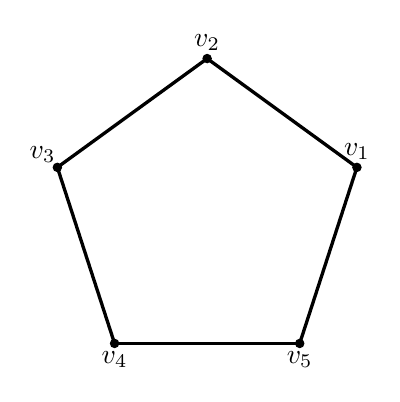
\begin{tikzpicture} 
\def \r {2 cm}
%\draw [dash pattern=on 1pt off 1pt, xstep=1cm,ystep=1cm] (-1,-2) grid (4, 2);
\begin{scope}[MyNodeStyle]  % 画点
\coordinate [label=above:$v_1$] (A) at (18:\r); \draw (A) node{}; 
\coordinate [label=above:$v_2$] (B) at (90:\r); \draw (B) node{}; 
\coordinate [label=above left:$v_3\,$]  (C) at (162:\r); \draw (C) node{}; 
\coordinate [label=below:$v_4$]  (D) at (234:\r); \draw (D) node{}; 
\coordinate [label=below:$v_5$]  (E) at (306:\r);  \draw (E) node{}; 
\end{scope}

\begin{scope}[MyEdgeStyle]  % 画边
\draw (A) to (B);
\draw (C) to (B);
\draw (D) to (C);
\draw (E) to (D);
\draw (E) to (A);
\end{scope}
\end{tikzpicture}
\caption{图的“图形”(用\LaTeX 画的)}
\label{FigG}
\end{center}
\end{figure}

\end{document}
